\documentclass[12pt]{report}

\usepackage[a4paper]{geometry}
%\geometry{left=2.5cm,right=2.5cm,top=2.5cm,bottom=2.5cm, a4paper}
\usepackage[utf8]{inputenc}
\usepackage{amsmath}
\usepackage{amsthm}
\usepackage{amssymb}
\usepackage{ulem}
\usepackage{graphicx}
\usepackage{caption}
\graphicspath{}
\usepackage[document]{ragged2e}
\usepackage{setspace}
\usepackage{tabularx}
\usepackage[slovene]{babel}
\usepackage{textcomp, gensymb}
\usepackage{siunitx}
\usepackage{pdfrender,xcolor}
\usepackage{hyperref}
\usepackage{xurl}
\usepackage{float}
\usepackage{titlesec}

\newfloat{slika}{htbp}{loc}
\floatname{slika}{Slika}

\newfloat{tabela}{htbp}{loc}
\floatname{tabela}{Tabela}

% Differential
\newcommand{\diff}{\mathrm{d}}

\title{
  
\includegraphics[width=0.4\textwidth]{fmf_logo}\\
  {\small Oddelek za fiziko} \\
  {Sevanje črnega telesa}\\
  {\small Poročilo pri fizikalnem praktikumu IV}\\

}
\date{}
\author{ Kristofer Č. Povšič \\[5 cm]
 \small  Asistentka: Jelena Vesić\\
}


\titleformat{\chapter}[hang]{\Huge\bfseries}{\thechapter{. }}{0pt}{\Huge\bfseries}

\setlength\parindent{0pt}

\begin{document}

\setcounter{page}{2}

\maketitle

\chapter*{Uvod}

Planckov zakon nam poda gostoto energije elektromagnetnega valovanja z neko frekvenco $\nu$ v votlini pri neki konstantni temperaturi $T$: 

\begin{equation}
  w( \nu, T) = \frac{8 \pi h \nu^3}{c^3} \frac{1}{\exp{\frac{h \nu}{kT}} - 1}
\end{equation}

kjer je $h$ Planckova konstanta in $c$ hitrost svetlobe v vakuumu. Skozi majhno luknjo te votline dobimo najboljši približek sevanja črnega telesa.

Z integracijo Planckovega zakona po frekvenci nam poda Stefanov zakon 

\begin{equation}
  \frac{P}{S} = \sigma T^4
\end{equation}

ki podaja moč, izsevano iz površine $S$ v celoten prostor. 

Prepustnost silicijevega filter, s katerim v drugem delu eksperimenta zastremo žarnico, lahko precej dobro opišemo kot stopničasto funkcijo, ki prepušča vse fotone z energijo manjšo kot $E_0 = 1.1 \si{eV}$. Analitično nerešljiv integral prepustnosti na prve 3 decimalke in s temperaturo $3000 \si{K}$ podaja naslednji približek 

\begin{equation}
  \frac{P'_{Si}}{P} \approx 1 - \frac{15}{\pi^4} \left[\ln(1 - e^{-y}) + e^{-y}(3y^2 + 6y +6)\right]
\end{equation}

Zaradi loma na površinah filtra imamo še dodatne izgube, ki jih lahko prestavimo s preprostim faktorjem 

\begin{equation}
  \eta = \frac{2n}{n^2 + 1}
\end{equation}

tako da je skozi filter zares prepuščena moč $P_{Si} = \eta P'_{Si}$. Pri tem je $n$ lomni količnik. 


\chapter*{Naloga}


\begingroup
\let\clearpage\relax
\begin{itemize}
  \item Izmerite odvisnost svetlobnega toka halogene žarnice v razponu od rahlega žarenja do maksimalne moči. Pri tem merite tudi moč, ki se troši na žarnici. 
  \item Narišite graf celotne izsevane moči kot funkcijo električne moči. 
  \item Določite električno upornost žarnice kot funkcijo temperature. 
  \item Narišite graf razmerja - skozi \verb+Si+ okno - prepuščenim in nemotenim svetlobnim tokom kot funkcijo temperature žarilne nitke. 
\end{itemize}



\chapter*{Potrebščine}
\begin{itemize}
\item merilec moči - wattmeter in električni multimeter 
\item halogena žarnica nazivne moči $30 \si{W}$ z nazivno barvno temperaturo $2700 \si{K}$
\item nastavljivi transformator - variac 
\item merilnik sevanja 
\item plošča iz kristalnega silicija. 
\end{itemize}

\chapter*{Navodilo}

Postavim vajo glede na navodila. Z multimetrom izmerim upornost žarilne nitke v žarnici pri sobni temperaturi. Halogeno žarnico priključim na variac, na katerem spreminjam napetost in posledično moč žarnice. Spreminjam moč žarnice v korakih po 5\% in si v tabelo zapisujem električno moč, tok in napetost na žarnici ter moč svetlobnega toka. Izmerim tudi moč sevanja, ki doseže detektor skozi okno iz kristalnega silicija, v odvisnost od moči žarnice v istem intervalu kot zgoraj in jo na grafu primerjam s teoretično napovedjo. 

\endgroup


\chapter*{Obdelava podatkov}

Žarnica se nahaja na razdalji 
\[
d = (74 \pm 1) cm
\]

Prostorski kot senzorja izražen z razdaljo in površino senzorja je: 

\begin{equation}
  \Omega = \frac{S}{d^2}
\end{equation}

kjer je $S = 1 \si{cm^2}$. Ko pomerim odvisnost na bolometru zaznane moči $P'(P_e)$ od električne moči, je celotna v prostor izsevana moč žarnice 
\begin{equation}
  P = \frac{P'}{\Omega}
\end{equation}

\begin{slika}[H]
  \centering
  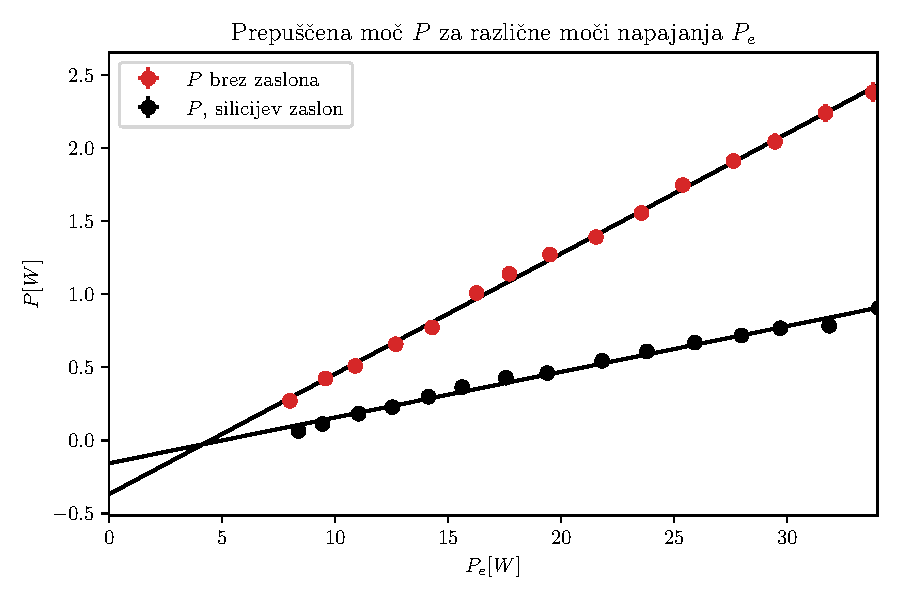
\includegraphics{PPe}
  \caption{\small Vsa v prostor izsevana moč žarnice pri različnih električnih močeh}
  \label{fig:PPe}
\end{slika}

Naklona premice sta 

\[
k_1 = 0.082 \pm 0.002 
\]
\[
k_2 = 0.031 \pm 0.002  
\]

in prvi naklon predstavlja izkoristek te žarnice. Z meritvijo tok in napetosti na žarnici in predpostavka, da ima žarnici pri moči $30 \si{W}$ temperaturo žarilne žice $T = (2700 \pm 100) \si{K}$. Upor žarilne žicke dobimo preko regresije, kjer velja enačba 

\begin{equation}
  R(T) = k_T T + R_0
\end{equation}

\begin{slika}[H]
  \centering
  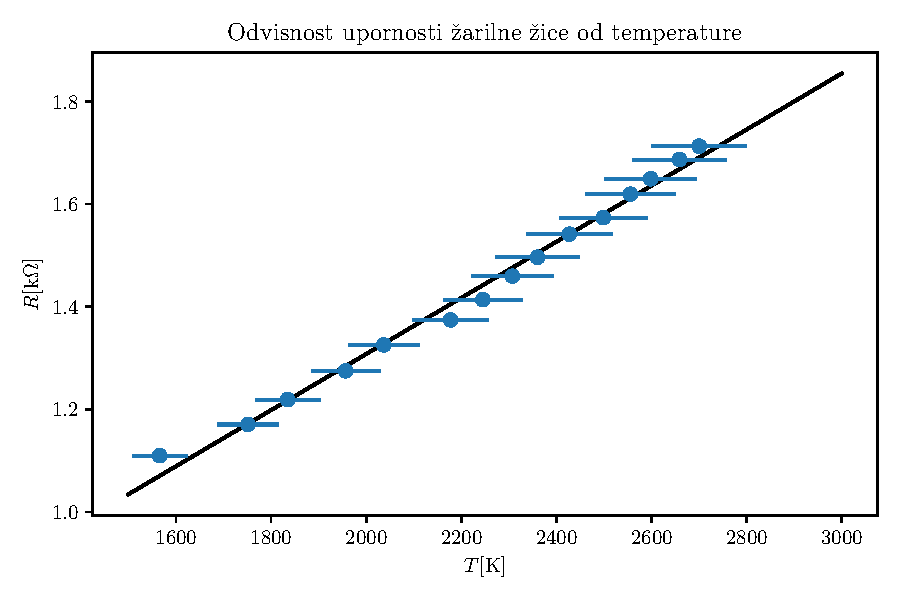
\includegraphics{RT}
  \caption{\small Graf prikazuje odvisnost upornosti žarilne žice od temperaturo z naklonom $k_T = 0.54 \pm 0.01$ in $R_0 = (210 \pm 30) \si{\Omega}$}
\end{slika}

Preverim še model za prepustnost silicijevega filtra. Ko jo prilagodimo meritvam, dobimo

\begin{slika}[H]
  \centering
  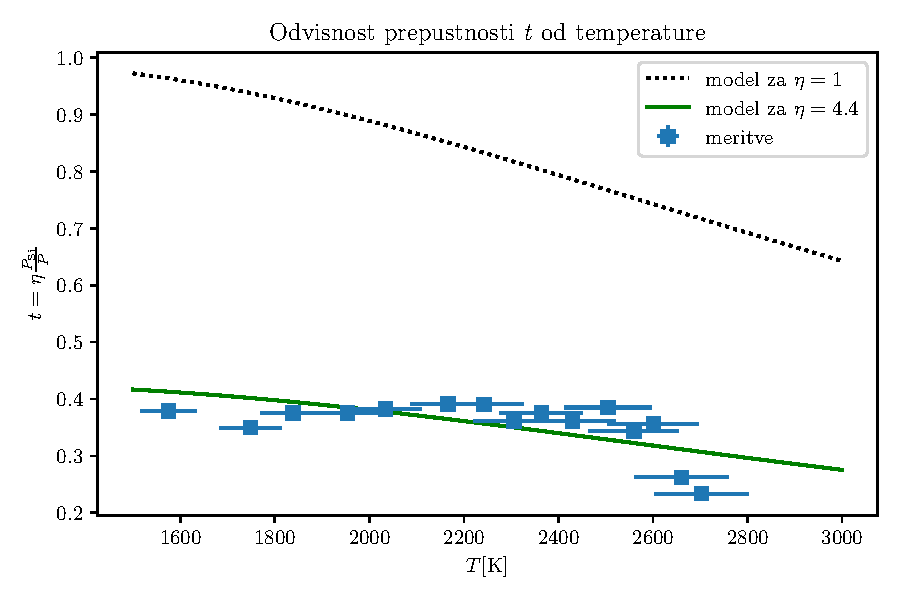
\includegraphics{tT}
  \caption{\small Izmerjene vrednosti prevodnosti s prilagojeno modelsko krivuljo (neprekinjena črta) in modelsko krivuljo, če ne bi upoštevali odbojev na površinah filtra (črtkana črta)}
\end{slika}

\[
\eta = 0.43 \pm 0.01  
\]

iz česar izračunamo še lomni količnik silicija 

\[
n = 4.4 \pm 0.1
\]


\end{document}